\documentclass{article}
\usepackage{style-assessments}

% define macros (/shortcuts)
\newcommand{\blankul}[1]{\rule[-1.5mm]{#1}{0.15mm}}	% shortcut for blank underline, where the only option needed to specify is length (# and units (cm or mm, etc.)))
\newcommand{\vecn}[2]{#1_1, \ldots, #1_{#2}}	% define vector (without parentheses, so when writing out in like a definition) of the form X_1, ..., X_n, where X and n are variable. NOTE: to call use $\vecn{X}{k}$ before parameters would go
\newcommand{\follow}[1]{\sim \text{#1}\,}		% shortcut for ~ 'Named dist ' in normal font with space before parameters would go
\newcommand{\followsp}[2]{\overset{#1}\sim \text{#2}\,}		% (followsp is short for 'follow special') shortcut that can be used for iid or ind ~ 'Named dist ' in normal font with space before parameters would go
\newcommand{\e}{\mathrm{e}}		% shortcut for non-italic e in math mode


\begin{document}

\hspace{375pt}Name:

\begin{center}
{\Huge MATH 321: Homework 6}
\end{center}

\bigskip\bigskip

{\large \textbf{Due} \blankul{4cm}: Turn in a hard copy, neat and stapled.}\bigskip

% problem types summary
% 1) exact t -> small n, normal, unknown var
% 2) exact t, pooled -> independent normal, common var, small n
% 3) approx t -> unknown dist and var, small n
% 4) approx z (one sample and two sample) -> large n, unknown dist (independent) and vars
% 5) approx t, pooled -> independent unknown dist and vars (check common)
% 6) approx t -> dependent samples, unknown dist and vars

Find the .xlsx file to work in and/or the .csv file to load into R on Canvas.\bigskip

For all the questions below, do the following:\bigskip
\begin{itemize}
    \item Choose the correct form of the interval, must provide justification for this choice (i.e. reference the variables that affect the scenarios we have discussed).
    \item Calculate the point estimate, critical value and standard error using technology (Excel / R).
    \item Give the final lower and upper bounds.
\end{itemize}\bigskip

\begin{enumerate}
    \item Assume that the yield per acre for a particular variety of soybeans is $N(\mu, \sigma^2)$ with unknown variance.
    \item[] Using the `Soybean' data, find an 80\% confidence interval for $\mu$.\bigskip%Lazar HW 5 AQ 2
    
    \item Let $X_1$ and $X_2$ equal be the earnings of two different stores owned by a toy company during the Christmas season. Assume that $X_1 \follow{N}(\mu_1, \sigma^2)$ and $X_2 \follow{N}(\mu_2, \sigma^2)$. Data is given in the excel file.
    \item[] Using the `Earnings' data, find a 95\% confidence interval for $\mu_1 - \mu_2$.\bigskip%Lazar HW 5 AQ 3 (except not using Welch's T, so changed setup to have common variance)
    
    \item As a clue to the amount of organic waste in Lake Macatawa, several samples of water were taken from the east basin and the count of the number of bacteria colonies in 100 milliliters of water was recorded.
    \item[] Using the `Bacteria' data, find a 90\% confidence interval for the mean number $\mu$ of colonies in 100 milliliters of water in the east basin.\bigskip%Prob and stat inference 7.1-5 (changed data so approx t instead of approx large sample z)
    
    \item SAT scores for 2010 are shown below. Separate random samples size 45 (so not the same test-taker's Verbal and Math) and produced the means and standard deviations listed in the accompanying table:%Math stats with apps problem 8.82
    \begin{figure}[H]
        \center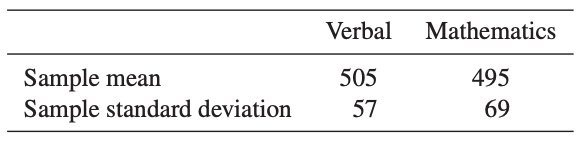
\includegraphics[scale=0.5]{images/data-SAT.png}
    \end{figure}
    \begin{enumerate}
        \item Construct a 92\% confidence interval for the mean Verbal score.
        \item Construct a 92\% confidence interval for the mean Math score.
        \item Construct a 92\% confidence interval for the mean difference in Verbal and Math scores.
        \item[] State a conclusion about how the mean Verbal and Math scores compare.
        \item Suppose the average scores in 2005 for Verbal and Math were 508 and 520, respectively. State a conclusion about how each score compares to the respective 2005 average.%Original addition
    \end{enumerate}\bigskip
    
    \item Researchers investigated a muscle condition between two types of exercise enthusiasts, runners and cyclists. Compartment pressure measurements were taken at for both groups at rest and during exercise (80\% max $O_2$ consumption). The data from random samples of 10 runners and 10 cyclists for compartment pressure (in millimeters of mercury) are summarized in the following table:%Math stats with apps problem 8.83
    \begin{figure}[H]
        \center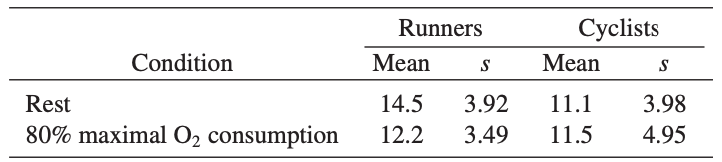
\includegraphics[scale=0.5]{Images/data-exercise.png}
    \end{figure}
    \begin{enumerate}
        \item Construct a 95\% confidence interval for the difference in mean compartment pressures between runners and cyclists under the resting condition.
        \item Construct a 90\% confidence interval for the difference in mean compartment pressures between runners and cyclists who exercise at 80\% of maximal oxygen (O2) consumption.
    \end{enumerate}\bigskip
    
    \item Twenty-four $9^{th}$ and $10^{th}$ grade high school girls were put on an ultraheavy rope-jumping program where their 40-yard dash times were measured before and after the program. Use the `40 yard dash time' data to:
    \begin{enumerate}%Stat inference problem 7.2-10 (generated data to match the differences so they have to do the differencing)
        \item Construct a 85\% confidence interval for the mean difference in before and after times for the 40-yard dash. State a conclusion about whether or not the jump rope program was effective.
        \item Construct a 98\% lower-bound confidence interval AND a 98\% upper-bound confidence interval for mean difference in before and after times for the 40-yard dash.%Original addition
        \item Combine the intervals from (b) to form a two-sided confidence interval. State the new confidence and the conclusion about whether or not the jump rope program was effective. Is this a different conclusion than in (a)?%Original addition
    \end{enumerate}
\end{enumerate}\bigskip



\vspace{50pt}

Select answers\bigskip
\begin{enumerate}
    \item $\approx [43.24, 53.16]$
    
    \item $\approx [218.76, 546.42]$
    
    \item $\approx [50.00, 75.47]$
    
    \item 
    \begin{enumerate}
        \item $\approx [490.12, 519.88]$
        \item $\approx [476.99, 513.01]$
        \item $\approx [-13.36, 33.36]$
        \item 
    \end{enumerate}
    
    \item 
    \begin{enumerate}
        \item $\approx [-0.31, 7.11]$
        \item $\approx [-2.62, 4.02]$
    \end{enumerate}
    
    \item 
    \begin{enumerate}
        \item $\approx [0.00, 0.16]$
        \item 
        \item $\approx [-0.03, 0.19]$
    \end{enumerate}
\end{enumerate}

\end{document}